\graphicspath{{./images/}}

\chapter{Bausteinsicht}

\section{Beschreibung}

Die Architektur für die Applikation wird mittel Schichten realisiert. Die Präsentationsschicht ist auf dem WebServer während sich die anderen vier auf dem AppServer befinden. Die einzelnen Komponenten wurden gruppiert um die Übersicht zu wahren. Auf der nächsttieferen Ebene sind diese Komponenten detaillierter aufgeführt.

\newgeometry{left=2.5cm, right=2.5cm, bottom=2.5cm, top=2.5cm}
\begin{landscape}
\section{Ebene 1 : Layer Architektur}

\begin{center}
	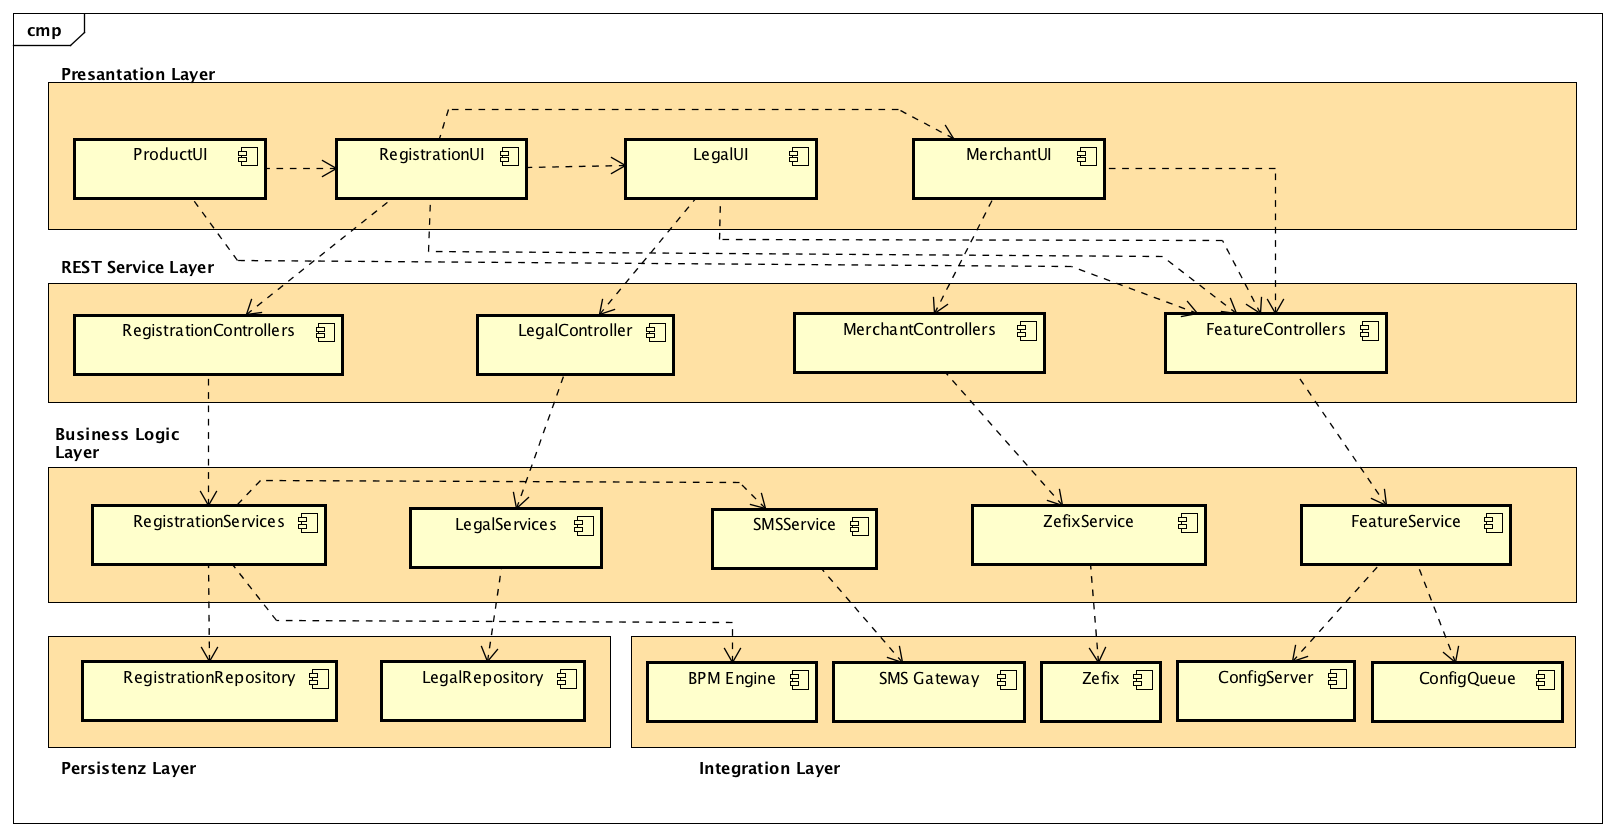
\includegraphics[scale=0.6]{ComponentLevel1.png}
\end{center}

\end{landscape}
\restoregeometry

\begin{table}[H]
	\centering
	\caption{Presentation Layer}
	\begin{tabular}{ | p{4cm} | p{11cm} | }
		\toprule
		{\textbf{Komponente}} & {\textbf{Beschreibung}} \\
		\midrule
		ProductUI &  Stellt die einzelnen Produktoptionen von Paymit dar welche der Benutzer auswählen kann\\ \hline
		RegistrationUI  &  Beinhaltet die Felder für den Start des Registrierungsprozesses sowie für die MTAN Verifikation.\\ \hline
		LegalUI &  Zeigt rechtliche Dokumente wie Allgemeine Geschäftsbedienungen an \\ \hline
		MerchantUI & Enthält das Formular für die Kooridinaten des Händler nach der erfolgreichen Verifikation des MTAN Codes und ist für den Abschluss der Registration zuständig.\\
		\bottomrule
	\end{tabular}
\end{table}

\begin{table}[H]
	\centering
	\caption{REST Service Layer}
	\begin{tabular}{ | p{4cm} | p{11cm} | }
		\toprule
		{\textbf{Komponente}} & {\textbf{Beschreibung}} \\
		\midrule
		RegistrationControllers &  Schnittstelle für den Start des Registrierungsprozesses. Startet den Prozess und fürt die Verifikation des MTAN Codes durch.\\ \hline
		LegalController &  Schnittstelle welche rechtliche Dokumente liefert \\ \hline
		MerchantController &  Schnittstelle für das Erfassen des Händler und Abschluss der Registration. \\ \hline
		FeatureControllers & Schnittstelle für das Abfragen der Features welche aktiv sind \\
		\bottomrule
	\end{tabular}
\end{table}

\begin{table}[H]
	\centering
	\caption{Business Logic Layer}
	\begin{tabular}{ | p{4cm} | p{11cm} | }
		\toprule
		{\textbf{Komponente}} & {\textbf{Beschreibung}} \\
		\midrule
		RegistrationService &  Enthält sämtliche Logik für die Aufbereitung der Registrierungsanfrage an die Workflow Engine. Für die Verifikation des MTAN Codes durch welcher via SMS versendet Wurde.\\ \hline
		LegalService &  Stellt die Dienste für das Abfragen den rechtlichen Dokumente bereit \\ \hline
		FeatureService &  Verwaltet die aktuell eingeschalteten Features welche aktiviert sind. Holt sich die neuen Konfigurationen automatisch nach einer Benachrichtigung durch die Message Queue. \\ \hline
		External Services & Schnittstelle zu diversen externen WebServices der Post, des Schweizer Bundes und des Handelsregister \\
		\bottomrule
	\end{tabular}
\end{table}

\begin{table}[H]
	\centering
	\caption{Persistenz Layer}
	\begin{tabular}{ | p{4cm} | p{11cm} | }
		\toprule
		{\textbf{Komponente}} & {\textbf{Beschreibung}} \\
		\midrule
		RegistrationRepository &  Speichert die Registrierungsdaten, den MTAN Code sowie die Requests, welche nicht direkt zur Workflow Enginge gesendet werden können. \\ \hline
		LegalRepository &  Holt die rechtlichen Dokumente aus dem Datenspeicher. \\
		\bottomrule
	\end{tabular}
\end{table}

\begin{table}[H]
	\centering
	\caption{Integration Layer}
	\begin{tabular}{ | p{4cm} | p{11cm} | }
		\toprule
		{\textbf{Komponente}} & {\textbf{Beschreibung}} \\
		\midrule
		Zefix &  Schnittstelle zum Download des Handelsregisterauszugs. \\ \hline
		UID &  Schnittstelle zur Unternehmensidentifikation anhand der UnternehmerID \\ \hline
		AddressChecker &  Schnittstelle zur Post für Addressverifikation und Autovervollständigung. \\ \hline
		Configserver &  Beinhaltet die Konfigurationen der einzelnen Featueres. \\ \hline
		SMS Gateway &  Sendet generierte Code an die vom Händler angegebene Nummer. \\ \hline
		ConfigeQueue & Message Queue welche die Benachrichtigungen für Konfigurationsänderungen enthält. \\ \hline
		BPM Engine & Verarbeitet die Registrierungsdaten im hinterlegten Workflow, beschrieben in Kapitel \ref{businesscase}\\
		\bottomrule
	\end{tabular}
\end{table}
\newpage


\section{Ebene 2 : RegistrationUI}
Anhand des Registrierungsintefaces soll der generelle Aufbau illustiert werden. Sämtliche UI Teile besitzen eine View in Form eines HTML Files. Der Controller steuert die Interaktion des Benutzers und sendet die Daten via Services an den REST Controller auf dem Server. Der FeatureService enthält Methoden um zu Prüfen ob einzelne Features im Interface aktiv sind oder nicht. Siehe dazu auch Kapitel \ref{toggles} Feature Toogles.

\begin{center}
	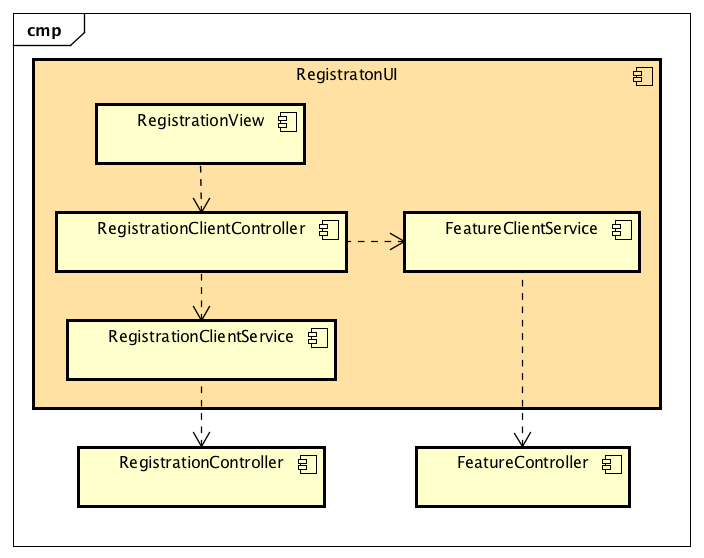
\includegraphics[scale=0.8]{WebComponentLevel2.png}
\end{center}
\newpage
\section{Ebene 2 : RegistrationServices}
\label{reg-service}

Der Registrierungsservice kümmert sich um die Aufbereitung der Daten für die Workflow Engine sowie die Übertragung der Daten. Er verwendet den SMS- und dem MailService um Nachrichten an den Händler zu schicken. Nach der Bestätigung des Benutzers, druch den MTAN Code, speichert er die Daten in der Datenbank. Der SchedulerService prüft regelmässig, ob neue Registierungen pendent sind, und sendet sie an die BPM Engine. Sollte bei der Kommunikation ein Fehler auftreten, wird zu einem späteren Zeitpunkt nochmals versucht die Daten an den Workflow zu schicken. 
\begin{center}
	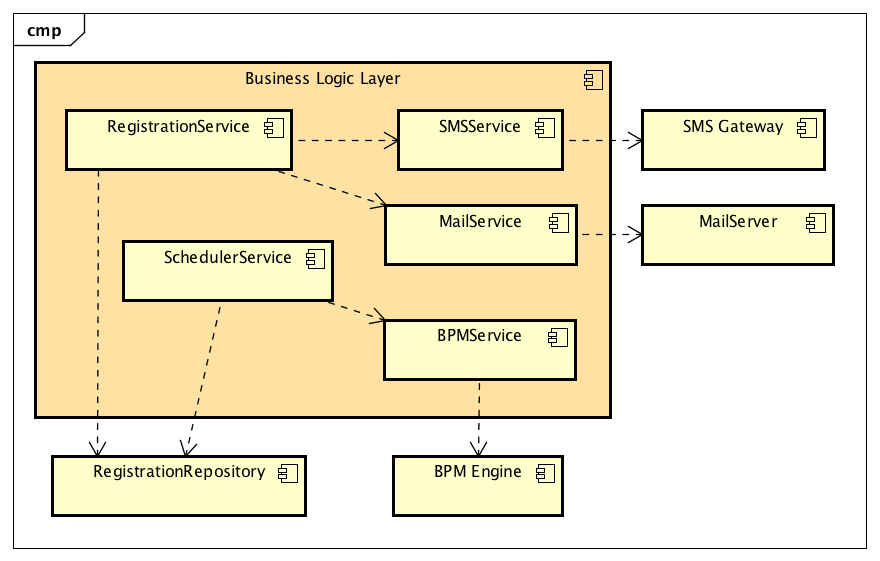
\includegraphics[scale=0.65]{RegistrationServicesLevel2.png}
\end{center}
\newpage
\section{Ebene 2 : ExternalServices}

Die ExternalServices bestehen aus den Diensten für die Unternehmensindentifikation, Handelsregisterauszug und Addressüberprüfungen. Sie erlauben eine vereinfachte Registierung des Händler welcher dadruch nicht alle Daten selber eingeben respektive zusammensuchen muss.

\begin{center}
	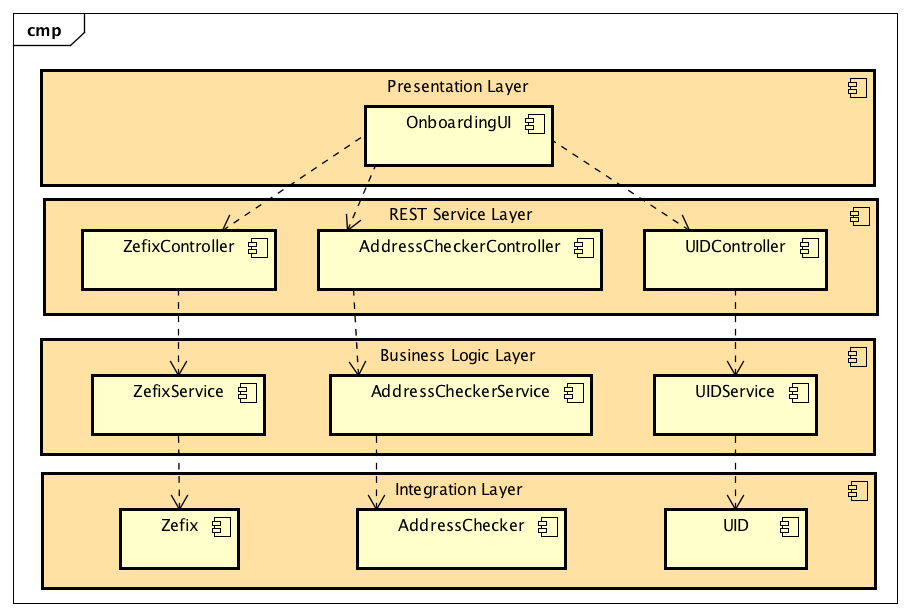
\includegraphics[scale=0.65]{ExternalServicesLevel2.png}
\end{center}

